%! Author = adnansiddiquei
%! Date = 08/03/2024

\section{Selection of Solution Algorithm and Prototyping}\label{sec:prototyping}
    \begin{figure}[htb]
    \centering
    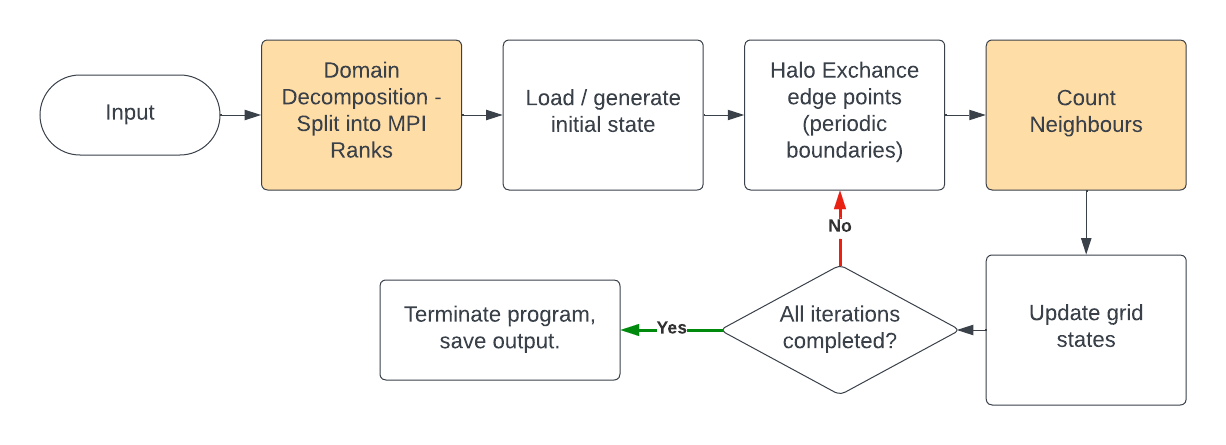
\includegraphics[width=0.9\textwidth]{./figures/high-level-flowchart}
    \caption{A high-level flow chart depicting the algorithm. The key points for efficiency considerations
    are highlighted in orange, the considerations are discussed in the main text.}
    \label{fig:high-level-flowchart}
    \end{figure}

    Fig.\eqref{fig:high-level-flowchart} shows the high-level algorithm being used to simulate Conway's
    Game of Life.
    The key points of consideration for efficiency are highlighted in orange.
    It is also worth noting that the rest of this section assumes that the grid is stored as a 1D array in row-major order.

    Domain decomposition can be done by either strips or blocks.
    Strips has the advantage that it is simpler to implement but will have more memory needing to be passed between
    boundaries, with the opposite being true for blocks.
    In the case of the neighbour counting algorithm, there are a couple of possible implementations.
    \begin{itemize}
        \item \textbf{Simple convolution.} Loop through each cell, and count the number of neighbours.
            This is equivalent to a 3x3 convolution with the below kernel.
            \begin{equation}
            \begin{bmatrix}
            1 & 1 & 1 \\
            1 & 0 & 1 \\
            1 & 1 & 1 \\
            \end{bmatrix}\label{eq:kernel1}
            \end{equation}
            This requires a total of $8N^{2}$ addition operations (the $9N^{2}$ multiplication operations that would usually occur can
            be ignored because the kernel only contain 1s and 0s so we can skip the multiplication operation in this special case).
        \item \textbf{Separable kernel.} If the following kernel is used instead,
            \begin{equation}
            \begin{bmatrix}
            1 & 1 & 1 \\
            1 & 1 & 1 \\
            1 & 1 & 1 \\
            \end{bmatrix}\label{eq:kernel2}
            \end{equation}
            then the kernel becomes separable.
            This means that the kernel can be split into two 1D identical kernels \(\begin{bmatrix} 1 & 1 & 1 \end{bmatrix}\) and
            applied in two passes which yields $2N^{2}$ addition operations per pass, yielding a total of $4N^{2}$ operations \cite{separable-kernel}.
            After another ${N^{2}}$ addition operations, to correct for replacing the central 0 with a 1, the total number of
            operations becomes $5N^{2}$.
            Therefore, the separable kernel method yields a theoretical speedup of $8/5 \approx 1.6$.
    \end{itemize}
    The simple convolution method introduces the issue of strided memory access when counting the 6 neighbours that are
    not horizontally adjacent to the current cell, as illustrated in Fig.\eqref{fig:neighbour-illustration}.

    \begin{figure}[htb]
    \centering
    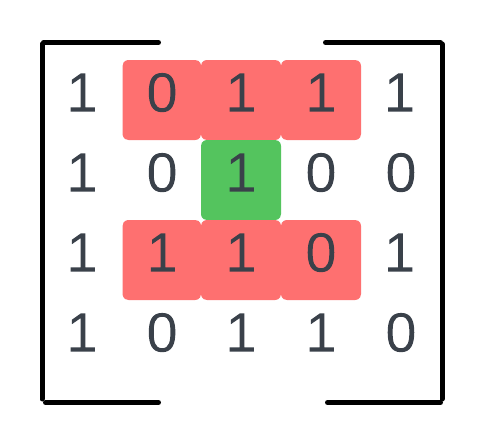
\includegraphics[width=0.35\textwidth]{./figures/neighbour-illustration}
    \caption{Illustration showing that the 6 vertical neighbours (highlighted in red) of the green cell are not contiguous
    in memory when representing a 2D array as a 1D array of points in row-major order.}
    \label{fig:neighbour-illustration}
    \end{figure}

    Therefore, when implementing the simple convolution method, column-wise decomposition would be preferred as it would 
    reduce the number of cache misses.
    This is because an $N \times N$ grid split into $P$ columns would yield a \inlinecode{N/P * sizeof(int)} byte distance
    between a cell and it's vertical neighbour whereas the same grid split into $P$ rows would yield a
    \inlinecode{N * sizeof(int)} byte distance, and $P$ blocks would yield a distance of yield
    \inlinecode{N/sqrt(P) * sizeof(int)} (assuming $P$ is a square number and $N$ is perfectly divisible by $P$).

    However, the separable kernel method does not have this issue as the data is contiguous on the horizontal pass,
    and the data can be made contiguous for the vertical pass by transposing the grid.
    Therefore, it does not matter which decomposition method is used for the separable kernel method with respect to cache
    misses.
    Furthermore, the type of domain decomposition used will also affect the speed of the transpose operation.
    If the transpose operation is done by writing contiguous and reading strided (which is generally faster), then column
    decomposition would be preferred as it would reduce the number of cache misses when reading the grid.

    However, which decomposition method is faster is still dependent on how the memory exchange rates between MPI ranks
    affects the overall performance of the algorithm, meaning both columns and blocks will need to be explored for efficiency.
    Likewise, a variety of OpenMP techniques will be used to multithread the convolution and transpose operation within
    each MPI rank, and various single thread optimisations will be explored to make use of SIMD vectorisation on the CPU level.
    These are all explored and the assumptions above are all tested in the next section to identify the optimal algorithm.


